\documentclass[conference]{IEEEtran}
\IEEEoverridecommandlockouts
% The preceding line is only needed to identify funding in the first footnote. If that is unneeded, please comment it out.
%Template version as of 6/27/2024

\usepackage{cite}
\usepackage{amsmath,amssymb,amsfonts}
\usepackage{amsthm}
\usepackage{algorithm}
\usepackage{algpseudocode}
% \usepackage{algorithmic}
\usepackage{graphicx}
\usepackage{textcomp}
\usepackage{xcolor}
\usepackage{threeparttable}
\usepackage{subcaption}
\usepackage[margin=1in]{geometry}
\def\BibTeX{{\rm B\kern-.05em{\sc i\kern-.025em b}\kern-.08em
    T\kern-.1667em\lower.7ex\hbox{E}\kern-.125emX}}
\begin{document}

\title{Data mining methods based on swarm intelligence to extract dense itemsets
}


\author{
  \IEEEauthorblockN{Anonymous Authors}\\
  \IEEEauthorblockA{Paper under double-blind review}
}

% \author{\IEEEauthorblockN{Taihei Takahashi\IEEEauthorrefmark{1}, Satoshi Suga\IEEEauthorrefmark{2} and Satoshi Kurihara\IEEEauthorrefmark{3}}
% \IEEEauthorblockA{\IEEEauthorrefmark{1}dept. name of organization (of Aff.)\\
% Email: email address or ORCID}
% \IEEEauthorblockA{\IEEEauthorrefmark{2}dept. name of organization (of Aff.)\\
% Email: email address or ORCID}
% \IEEEauthorblockA{\IEEEauthorrefmark{3}dept. name of organization (of Aff.)\\
% Email: email address or ORCID}
% }



\maketitle

\begin{abstract}
% This study proposes new two methods for dense pattern extraction. In transaction data, the frequency of occurrence of some patterns increases during a specific period of time, and important events or factors may be hidden behind them. Conventional methods typically focus on evaluating the rate of occurrence in the entire data, making it challenging to capture local variations. As an alternative, we propose Apriori-window, an exact solution method using a sliding window mechanism, and Plant Model, a heuristic method based on a swarm intelligence algorithm. Experiments on real data show that the proposed methods have the same or higher pattern extraction accuracy than existing methods.

Numerous methods have been proposed for frequent itemset mining. Transaction data often exhibits patterns whose occurrence frequencies increase during specific time intervals, potentially indicating important underlying events or factors. Conventional methods typically focus on support over the entire dataset, making local variations difficult to capture. As alternatives, this paper proposes Apriori-Window, an exact solution leveraging a sliding-window mechanism, and Plant Model, a heuristic based on a swarm intelligence algorithm. Experiments on real data demonstrate that the proposed methods achieve pattern-extraction accuracy comparable to or better than existing methods.
\end{abstract}

\begin{IEEEkeywords}
data mining, swarm intelligence, time series data, frequent pattern mining.
\end{IEEEkeywords}

\section{Introduction}
\label{introduction}

Recent increases in the volume of transaction data have rendered data analysis indispensable across diverse fields. The dynamic nature of data patterns, which often change over time, necessitates methods that can capture local variations. Transactions occurring with high frequency during specific intervals may reflect underlying factors such as seasonality, promotional activities, or societal trends. Detecting these dense patterns enables the extraction of significant insights, thereby facilitating effective decision-making and strategic planning.

Extracting dense patterns is challenging because it requires assessing the local frequency variations of itemsets rather than relying solely on global frequency metrics. Although numerous methods for itemset extraction exist \cite{agrawal1994fast}\cite{zaki1997new}\cite{han2000mining}, they primarily focus on overall frequency and fail to capture local fluctuations. Methods that consider the gaps between itemset occurrences have been proposed \cite{tanbeer2009discovering}\cite{kiran2017discovering}\cite{mahanta2005finding}\cite{fournier2021mining}, but our preliminary experiments revealed that their extraction accuracy is highly sensitive to the maximum allowed gap parameter. Moreover, these approaches do not exhaustively extract all dense patterns.

To address these issues, we propose two novel methods. The first method, termed \emph{Apriori-window}, is an exact solution that leverages a sliding window mechanism to evaluate local frequency variations without the need for a fixed maximum gap parameter. While this approach guarantees high extraction accuracy, its computational cost increases when itemsets occur frequently due to the exhaustive scanning of all occurrence points.

The second method, referred to as the \emph{Plant Model}, is an approximate solution that implements a swarm intelligence algorithm to detect dense intervals. By limiting scanning to these regions, the Plant Model reduces computational overhead while maintaining a robust performance. Together, these methods overcome the limitations of existing approaches by mitigating parameter sensitivity and reducing computational costs, thereby enabling efficient and accurate extraction of dense patterns from transaction data.

In Section 2 of this paper, we review related research on frequent itemset mining, variable frequency extraction, and swarm intelligence applications. Section 3 defines the problem. In Section 4, we present the proposed methods, \emph{Apriori-window} and the \emph{Plant Model}. Section 5 details the experimental setup, results, and discussion. We conclude in Section 6 with a brief summary and mention of future research directions.

\section{Related Works}
\label{related_works}

Methods for extracting itemsets from data have been extensively studied in the field of itemset mining \cite{fournier2017survey}. Various pattern evaluation methods and extraction techniques have been proposed based on the specific characteristics of the itemsets. Recent trends in itemset and pattern mining are summarized in \cite{fournier2022pattern} and \cite{fournier2019survey}.

A representative task in this domain is frequent itemset mining, which involves extracting itemsets that appear often in the dataset. Methods such as Apriori \cite{agrawal1994fast}, ECLAT \cite{zaki1997new}, and FP‑Growth \cite{han2000mining} have been developed for this purpose. In contrast, dense patterns are itemsets that exhibit high frequency within specific intervals despite having low overall support. The aforementioned methods evaluate only global frequency and fail to capture local variations. As a result, a high minimum support threshold may overlook low‑frequency dense patterns, while a low threshold expands the search space with many non‑dense patterns—a dilemma known as the rare item problem \cite{liu1999mining}.

To overcome these challenges, research has focused on extracting patterns based on variations in frequency over time. For example, TP‑Mine \cite{wan2009discovering} extends an earlier method \cite{dong1999efficient} by splitting the data at a specified point and extracting itemsets with significant frequency changes between the resulting halves. However, the extracted patterns depend heavily on the chosen split point. SPF \cite{chang2002mining} calculates an itemset’s frequency over the span from its first to its last occurrence to identify high‑frequency segments; however, it cannot capture finer‑grained frequency changes within that span.
% limiting its ability to extract patterns that appear briefly but intensely.

As alternatives, methods based on the gaps between itemset occurrences have been proposed \cite{radhakrishna2015survey}. Periodic Frequent Pattern Mining(PFPM) \cite{tanbeer2009discovering} extracts itemsets that occur frequently overall and whose every gap between successive occurrences does not exceed a preset maximum gap. Although a short maximum gap can define density, it excludes dense patterns with variable spacing. Partial Periodic Frequent Pattern Mining(PPFPM) \cite{kiran2017discovering} relaxes this constraint by introducing a threshold on the ratio of gaps that meet the maximum gap. However, since it does not require these gaps to be consecutive, it cannot reliably distinguish truly dense intervals from sparse ones. Additionally, methods such as Locally Periodic Frequent Itemset Mining(LPFIM) \cite{mahanta2005finding} and Local Periodic Pattern Mining(LPPM) \cite{fournier2021mining} search for runs of occurrences in which each gap is below the maximum and the run length satisfies a minimum requirement. LPFIM, for example, identifies each contiguous run of occurrences whose gaps all lie beneath the threshold and whose length meets a minimum; its accuracy, however, is highly sensitive to the chosen gap threshold: if set too high, intervals become too long and dilute the local density; if too low, they fragment and fail to capture true bursts. Similarly, LPPM accumulates the difference between each gap and the maximum gap until a threshold is exceeded, but a high allowance admits non‑dense intervals and lowers precision. Overall, these gap‑based methods struggle to handle diverse periodicities while maintaining high extraction accuracy.

Swarm intelligence \cite{kennedy2006swarm} has been applied to reduce the computational cost of pattern evaluation through localized search. Swarm intelligence involves multiple agents cooperating to solve optimization problems and is embodied in algorithms such as Particle Swarm Optimization (PSO) \cite{kennedy1995particle} and Genetic Algorithms (GA) \cite{holland1975adaptation}. In these approaches, many agents explore the solution space, and the search narrows based on provisional optimal solutions, enabling rapid convergence to near‑optimal results. Pattern mining can be viewed as an optimization problem where the evaluation metric serves as the objective function and the extracted patterns are the solutions. Consequently, swarm intelligence techniques have been applied to pattern mining \cite{djenouri2018new}\cite{telikani2020survey}. Extensions of PSO for pattern mining, such as PSO‑FIM \cite{kuo2011application} and PSO‑Apriori \cite{djenouri2017combining}, represent each particle’s position as an itemset and update these positions based on evaluation values. Similarly, GA‑based methods such as AGA \cite{alatacs2006efficient}, GA‑FIM \cite{djenouri2014association}, and GA‑Apriori \cite{djenouri2017combining} evolve itemset representations through selection, crossover, and mutation. Although these swarm intelligence methods reduce the number of candidate patterns, they still require scanning the entire dataset for evaluation, which limits the overall efficiency.

The proposed approach distinguishes itself from existing works in two key aspects. First, it redefines dense patterns by removing any gap constraint from their definition of support, thereby eliminating difficult gap‑threshold tuning and enabling more accurate extraction. Second, it incorporates an agent‑based local search that focuses on dense intervals without scanning the entire dataset. By restricting evaluation to these spans, we can significantly reduces computational costs while preserving the accuracy.

\section{Problem Definition}
\label{probelm_def}
\subsection{Terminology}
An itemset is a set of items, written as \( i_{j_1}\ i_{j_2}\ \dots\ i_{j_k} \). The length of an itemset refers to the number of items it contains. A transaction is defined as a pair \((ts, X)\), where \(ts\) is a timestamp (an integer representing the time of occurrence) and \(X\) is an itemset. A list of transactions is called transaction data, denoted by \(D = [d_1, \dots, d_N]\). The length of the transaction data is the number of transactions it contains. In this study, we focus on data in which timestamps are recorded at fixed intervals.

We arrange the timestamps of each transaction in ascending order to form a list without duplicates,\(T = [ts_1, \dots, ts_N].\)
In this paper, a \emph{gap} denotes the distance between two successive occurrences of the same itemset in \(T\): if \(P\) appears at positions \(p_k\) and \(p_{k+1}\), then $  \mathit{gap} \;=\; p_{k+1} - p_k,$
which may exceed one when those occurrences are not adjacent. An \emph{interval}, by contrast, is the contiguous span defined by its start and end timestamps \([ts_i, ts_j]\) (with \(1 \le i \le j \le N\)), whose length is \(j - i + 1\). We denote by $D_I = [X_{ts_i}, \dots, X_{ts_j}]$ the list of itemsets corresponding to all transactions within this interval, and write its length as $n(D_I)$.

To identify itemsets that are dense within specific intervals, we use the interval support proposed by \cite{mahanta2005finding} as a measure of local occurrence frequency. Specifically, for an interval \(I = [ts_i, ts_j]\), the interval support of an itemset \(P\), denoted by \(Sup_I(P)\), is defined by Equation (\ref{eq:support}):

\begin{IEEEeqnarray}{rCl}
Sup_I(P)
= \frac{n\bigl(\{\,X\in D_I \mid P\subseteq X\,\}\bigr)}{n(D_I)}
\label{eq:support}
\end{IEEEeqnarray}
where \(D_I\) and \(n(\cdot)\) are as defined above.

In contrast to the support defined in frequent itemset mining \cite{agrawal1994fast}, which is normalized by the total length of the dataset, the interval support is normalized by the length of each interval \(I\) and thus measures the local frequency. Given thresholds \(minSup\) (minimum interval support) and \(minL\) (minimum interval length), we call an interval \(I = [ts_i, ts_j]\) a dense interval for an itemset \(P\) if it satisfies:

\begin{enumerate}
    \item \(Sup_I(P) \ge \textit{minSup}\), and  
    \item \((j - i + 1) \ge \textit{minL}\).
\end{enumerate}

% When listing dense intervals in ascending order of their timestamps, we denote the \(k\)-th such dense interval for \(P\) by \(CI_k^P\). 
If an itemset \(P\) has at least one dense interval, then \(P\) is called a dense pattern. Intuitively, \(\textit{minSup}\) determines whether the pattern appears sufficiently often in a given interval, while \(\textit{minL}\) enforces a minimum duration. A low \(\textit{minL}\) makes the method sensitive to brief bursts, whereas a high \(\textit{minL}\) smooths out short fluctuations and captures longer trends.

\subsection{Preliminary Experiments:Performance Issues}


\begin{figure}[t]
    \centering
    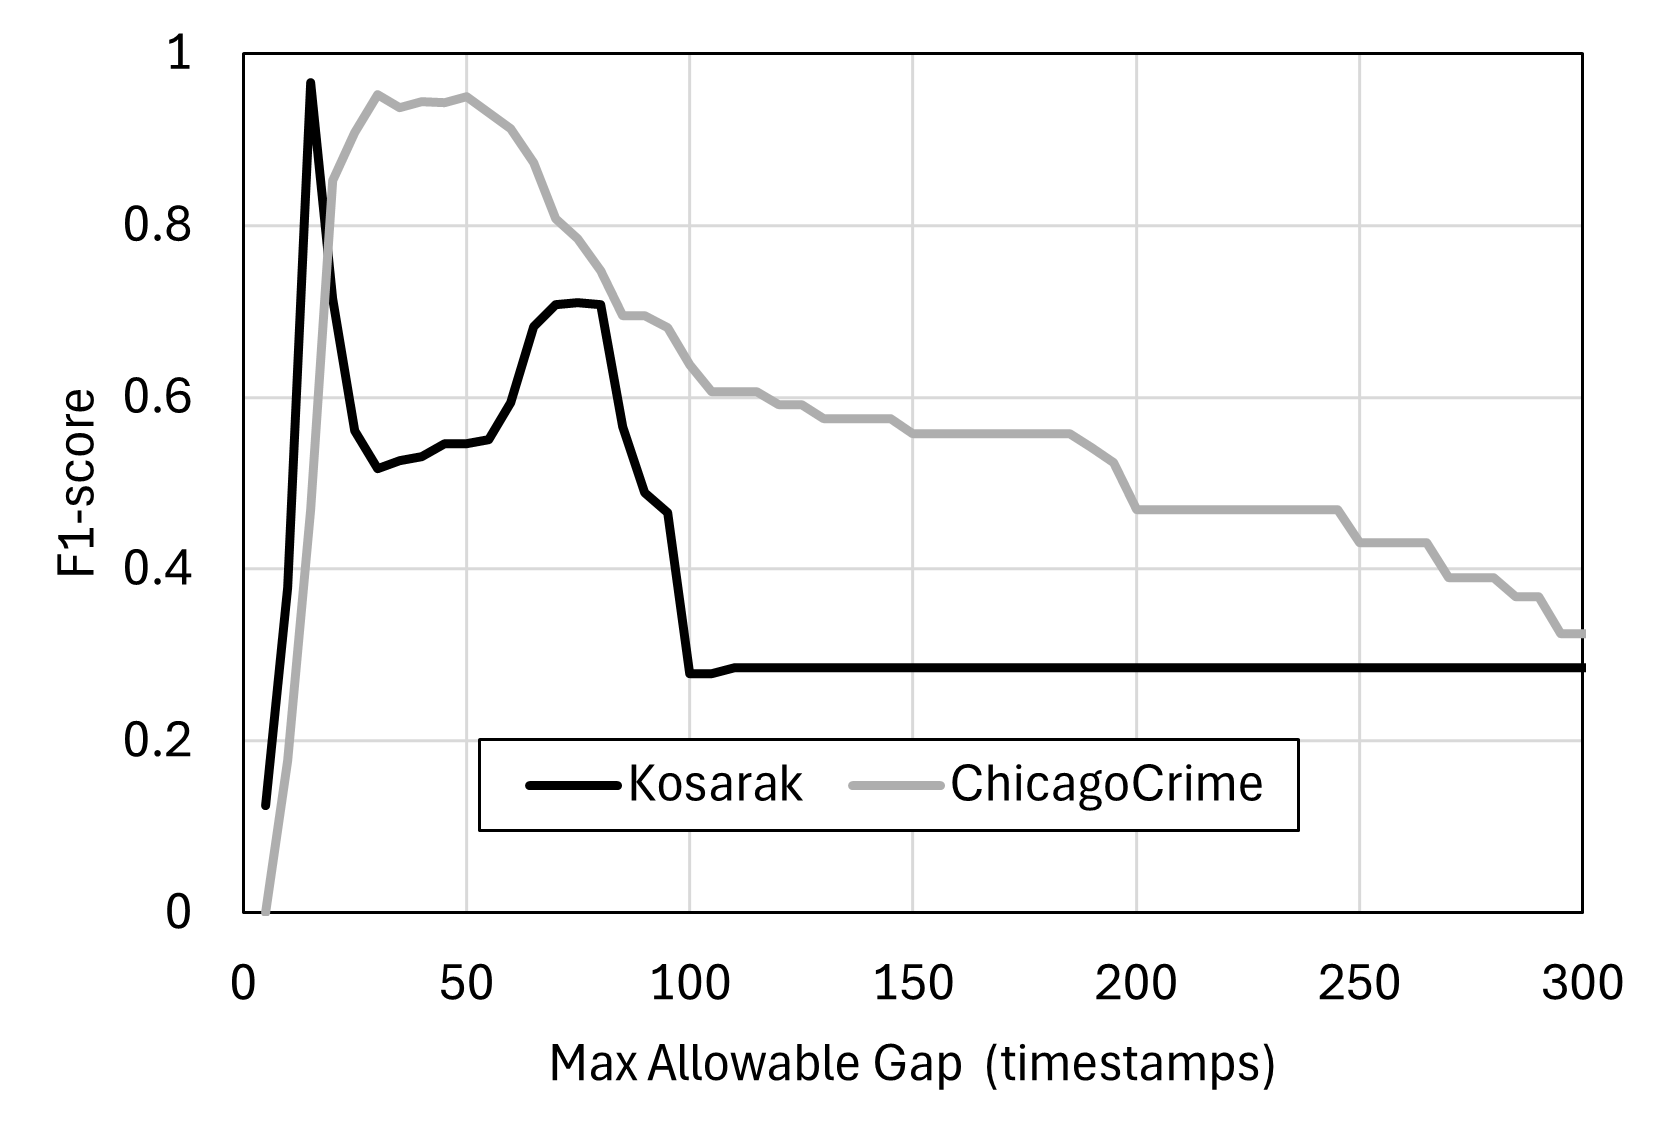
\includegraphics[width=1\linewidth]{fig/preliminary.png}
    \caption{Variation of extraction accuracy according to the maximum allowable gap when LPFIM is applied to extract dense patterns.The x-axis is the max allowable gap and the y-axis is the F1-score. This line indicates that the threshold setting of the max allowable gap affects the accuracy of the pattern detection.}
    \label{fig:acc_of_related_works}
\end{figure}

We conducted preliminary experiments to clarify the issues that arise when applying LPFIM\cite{mahanta2005finding} to the dense pattern extraction task. In these experiments, LPFIM was applied to two real-world datasets while the maximum allowable gap—a key parameter—was varied in increments of 5, and the resulting F1-scores were measured. Statistical details of the datasets are provided in Section \ref{sec:experiments}.

The target dense patterns were predetermined as ground truth. In the comparison between the ground truth and the itemsets extracted by LPFIM, we define recall as the fraction of ground-truth patterns covered by the extracted itemsets, precision as the fraction of extracted itemsets that correspond to true dense patterns, and compute the F1-score based on these two metrics (see Equations (\ref{eq:recall}), (\ref{eq:precision}) and (\ref{eq:f1score}) below).

\begin{IEEEeqnarray}{rCl}
Recall & = & \frac{\lvert A\cap G\rvert}{\lvert G\rvert}\,, 
\label{eq:recall}\\
Precision & = & \frac{\lvert A\cap G\rvert}{\lvert A\rvert}\,, 
\label{eq:precision}\\
F1\text{-}score & = & \frac{2\,\lvert A\cap G\rvert}{\lvert G\rvert + \lvert A\rvert}\,. 
\label{eq:f1score}
\end{IEEEeqnarray}


% For the preliminary experiments, the parameter settings were as follows: for the Kosarak, and ChicagoCrime datasets, the minimum interval length was 250 with a minimum interval support of 0.1.
For these preliminary experiments, the ground-truth dense patterns were generated using the following settings: for both the Kosarak and ChicagoCrime datasets, a minimum interval length of 250 and a minimum interval support of 0.1. The LPFIM algorithm parameters are detailed in Appendix \ref{sec:params}.

Fig.~\ref{fig:acc_of_related_works} presents the experimental results. It is evident here that the extraction accuracy is sensitive to the setting of the maximum allowable gap, with particularly high F1-scores observed for these datasets only within a specific range. These findings imply that, when applying existing methods to the dense pattern extraction task, the maximum allowable gap must be carefully tuned to an optimal range—a process that is inherently challenging.

In light of these issues, we propose a novel method aimed at mitigating the difficulty of parameter tuning while simultaneously enhancing the accuracy of dense pattern extraction.
\section{Proposed Method}
\label{proposed_method}
\subsection{Apriori-window}
Dense patterns denote itemsets with high local occurrence frequencies. 
It is impractical to determine whether a pattern is dense for all combinations of items that appear in transaction data due to combinatorial explosion. 
Therefore, it is necessary to limit the target of pattern evaluation to a set of itemsets whose occurrences are locally concentrated. 
The method exploits Apriori’s anti-monotonicity\cite{agrawal1994fast}: if an itemset fails to meet the minimum interval support ($minSup$) and minimum interval length ($minL$) criteria, every superset thereof is automatically invalid. By leveraging this property, the conventional Apriori framework is adapted for dense pattern extraction, resulting in the exact algorithm \emph{Apriori-window} that exhaustively enumerates these patterns.
We prove below that anti-monotonicity holds in dense patterns.

\begin{proof}[Proof of the Anti-monotonicity in Dense Patterns]
Let \( D = [d_1, \dots, d_N] \) be a transaction dataset with each transaction represented as \( d_i = (ts_i, X_{ts_i}) \), and let the ordered list of timestamps be \( T = [ts_1, \dots, ts_N] \). For any interval \( I = [ts_i, ts_j] \) with length $n(D_I) = j - i + 1 \ge \textit{minL}$,
denote the corresponding sequence of itemsets by
$D_I = [X_{ts_i}, \dots, X_{ts_j}]$.

Assume that an itemset \( P \) is not a dense pattern; that is, for every interval \( I \) with \( n(D_I) \ge \textit{minL} \), we have
$Sup_I(P) < \textit{minSup}$.
Consider any extension \( P' \) such that \( P \subset P' \). For any interval \( I \), define
$T(P'; I) = \{ X \in D_I \mid P' \subseteq X \}$
as the set of transactions in \( I \) containing \( P' \), and similarly define
$T(P; I) = \{ X \in D_I \mid P \subseteq X \}$.
Since every transaction that contains \( P' \) also contains \( P \), it follows that
$T(P'; I) \subseteq T(P; I)$.
Thus, we have
$n\bigl(T(P'; I)\bigr) \le n\bigl(T(P; I)\bigr)$,
which implies
\[
Sup_I(P') = \frac{n\bigl(T(P'; I)\bigr)}{n(D_I)} \le \frac{n\bigl(T(P; I)\bigr)}{n(D_I)} = Sup_I(P).
\]
Consequently, for every interval \( I \) with \( n(D_I) \ge \textit{minL} \),
\[
Sup_I(P') \le Sup_I(P) < \textit{minSup}.
\]
Furthermore, since the occurrence positions of \( P' \) form a subset of those of \( P \), if no contiguous interval of length at least \(\textit{minL}\) exists for \( P \) (i.e., no \( I \) with \( n(D_I) \ge \textit{minL} \) satisfies \( Sup_I(P) \ge \textit{minSup} \)), then none exists for \( P' \) either.

Therefore, any extension \( P' \) of an itemset \( P \) that is not a dense pattern will necessarily fail to meet the conditions
\[
Sup_I(P') \ge \textit{minSup} \quad \text{and} \quad n(D_I) \ge \textit{minL},
\]
thereby establishing the anti-monotonicity of dense patterns.
\end{proof}



\begin{algorithm}[t]
    \makeatletter
    \renewcommand{\algorithmicrequire}{\textbf{Input:}}
    \renewcommand{\algorithmicensure}{\textbf{Output:}}
    \makeatother
    \begin{algorithmic}[1]
    \caption{Main Algorithm of Apriori-window}
    \label{alg:apriori-window}
        \Require Dataset $D$, minimum interval support $minSup$, minimum interval length $minL$
        \Ensure Set of dense patterns $L$ and their occurrence intervals
        \State $L \gets \{\}$
        % \Comment{Initialize the set of dense patterns}
        \State Evaluate each single item by sliding window mechanism.
        \State Add the length-$1$ dense pattern and its dense intervals to $L(1)$.
        \For{$k \gets 2$ \textbf{to} $L(k-1) \neq \emptyset$}
            \State $L(k) \gets \{\}$
            \State $C_k \gets \{\}$ 
            % \Comment{Initialize the candidate set for itemsets of length $k$}
            \State Generate all candidate itemsets of length $k$ from $L(k-1)$.
            \State Add the candidate itemsets to $C_k$.
            \For{each candidate in $C_k$}
                \State Evaluate the candidate by the sliding window mechanism.
                \State Add the length-$k$ dense patterns and its dense intervals to $L(k)$.
            \EndFor
        \EndFor
        \State \Return $\bigcup_k L(k)$
    \end{algorithmic}
\end{algorithm}


Algorithm~\ref{alg:apriori-window} presents the core procedure of the Apriori-window algorithm. In the initial phase, the algorithm scans the occurrence positions of each item using a sliding window mechanism. This mechanism utilizes a fixed-width window that moves sequentially over the transaction data, precisely capturing local frequency variations. Within each window, it evaluates the occurrence frequency of items and merges overlapping dense intervals, thereby extracting dense single-item patterns.A detailed description of the sliding window mechanism is provided in Algorithm~\ref{alg/sliding_window_mechanism}.

Subsequently, candidate patterns of length two or more are generated by leveraging the Apriori property based on these dense single-item patterns. Each candidate is then assessed by the same sliding window mechanism, ensuring that local density is accurately measured while redundant evaluations are minimized.

Moreover, the module incorporates a stride adjustment technique (lines 17 to 19 in Algorithm \ref{alg/sliding_window_mechanism}) to enhance computational efficiency. When the support within a window exceeds the threshold, the surplus is used to determine an increased stride, thereby allowing the algorithm to skip redundant windows. 

\begin{algorithm}[t] 
    \caption{Sliding Window Mechanism} 
    \label{alg/sliding_window_mechanism}

    \makeatletter 
    \renewcommand{\algorithmicrequire}{\textbf{Input:}} 
    \renewcommand{\algorithmicensure}{\textbf{Output:}} 
    \makeatother
    
    \begin{algorithmic}[1] 
        \Require Occurrence positions for all items $positions$, itemset $X$, minimum interval support $minSup$, minimum interval length $minL$ 
        \Ensure List of dense intervals $C$ for the itemset $X$
    
        \State $W \gets minL$ 
        % \Comment{Set the width of the sliding window} 
        \State $positions(X) \gets$ List of occurrence positions of itemset $X$ (sorted in ascending order)
        \State $C \gets$ Empty list 
        % \Comment{Initialize the list of dense intervals}
        
        \For{$i \gets 0$ to $|positions(X)| - W -1$} 
            \State $window_{start} \gets positions(X)[i]$ 
            \State $window_{end} \gets window_{start} + W$ 
            \State $count \gets 0$ 
            \For{$j \gets i$ to $|positions(X)| - 1$} 
                \If{$positions(X)[j] < window_{end}$} 
                    \State $count \gets count + 1$ 
                \Else 
                    \State \textbf{break} 
                \EndIf 
            \EndFor 
            \If{$\dfrac{count}{W} \geq minSup$} 
                \State Add dense interval $[window_{start}, window_{end}]$ to $C$
                \State $surplus \gets support - minSup$ 
                % \Comment{Calculate the surplus of the interval support}
                \State $skip \gets \text{floor}(W \times surplus)$ 
                % \Comment{Obtain the integer part of the surplus using the floor function}
                \State $i \gets i + \max(1, skip) - 1$ 
                % \Comment{Determine the starting position of the next window}
            \EndIf
        \EndFor
        
        \State $C \gets$ Merge overlapping or adjacent dense intervals 
        \State \Return $(X,~C)$
        
    \end{algorithmic} 
\end{algorithm}


\subsection{Plant Model}
% We propose \emph{Plant Model} as a novel approach for extracting densely occurring patterns. 
% We implement a \emph{candidate extraction module} inspired by swarm intelligence to efficiently extract pairs of dense itemset candidates and their dense interval candidates.
% Subsequently, we apply a \emph{pattern evaluation module} to rigorously detect the dense intervals for each candidate, thereby identifying the dense patterns.
% The candidate extraction module and the pattern evaluation module are iteratively executed to output all extracted dense patterns and their dense intervals at the end of the process.


We propose the \emph{Plant Model} as a novel approach for extracting densely occurring patterns. It consists of two main components: a \emph{candidate extraction module}, inspired by swarm intelligence, and a \emph{pattern evaluation module} for rigorously detecting dense intervals. Fig.~\ref{fig:entire-flow} shows the flow chart of the proposed Plant Model.
The candidate extraction module extracts pairs of dense itemset candidates and their corresponding dense interval candidates. Subsequently, the pattern evaluation module applies rigorous detection to each candidate, thereby identifying the dense patterns. These modules are iteratively executed executed to output all extracted dense patterns and their dense intervals at the end of the process.

\begin{figure}[t]
    \centering
    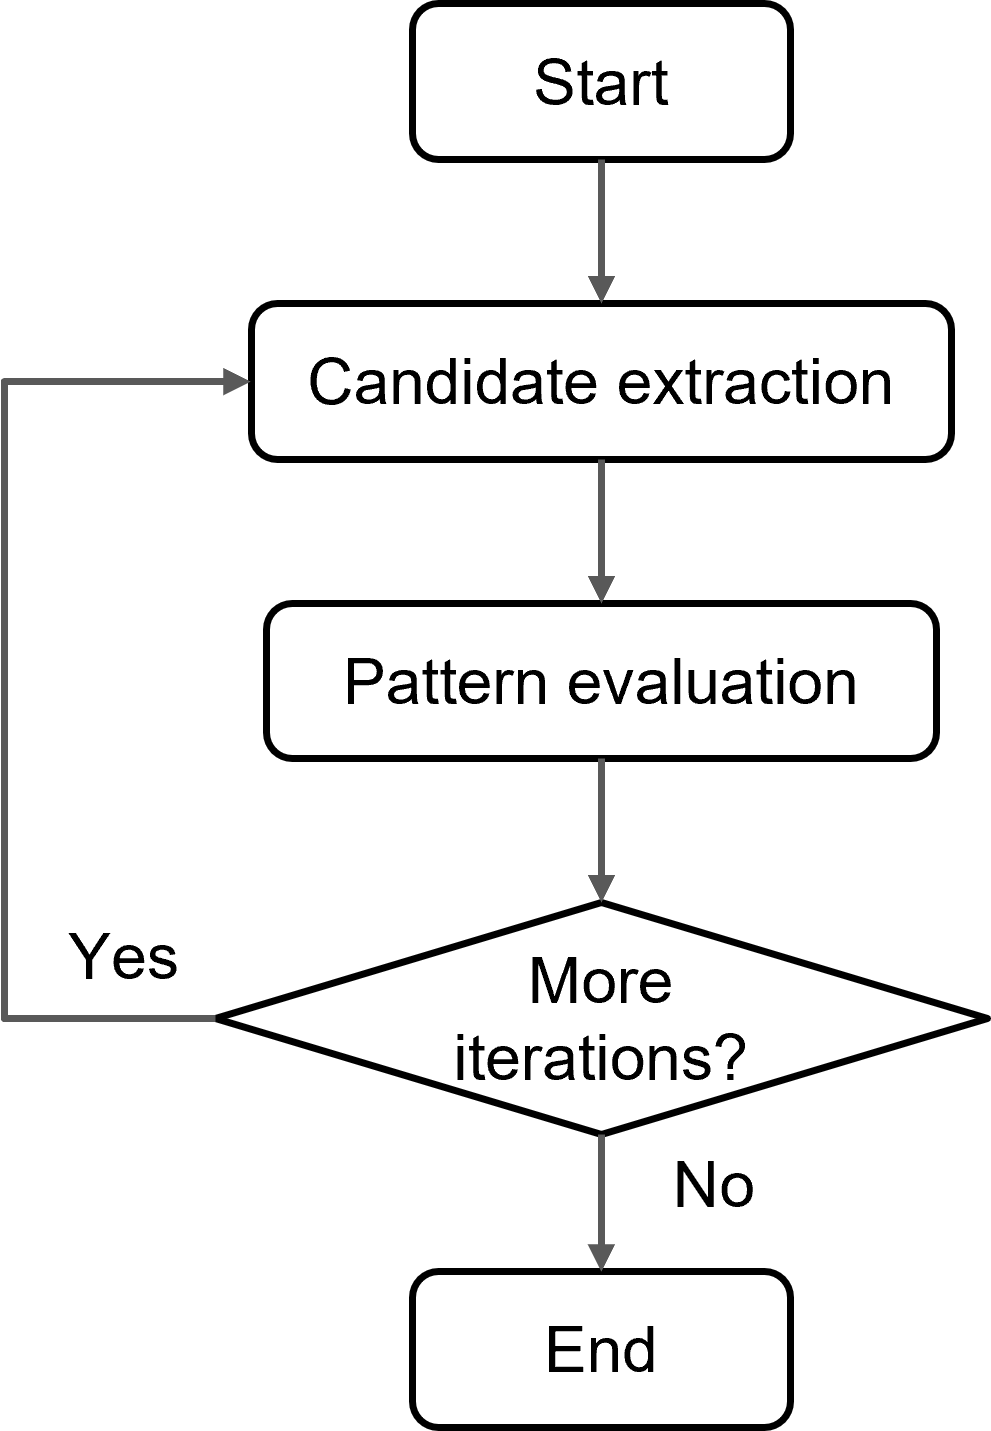
\includegraphics[width=0.5\linewidth]{fig/entire_flow.png}
    \caption{Flow chart of proposed Plant Model. The candidate extraction module and the pattern evaluation module are executed in sequence and repeated until the early termination condition is satisfied or the maximum number of iterations is reached.}
    \label{fig:entire-flow}
\end{figure}

\subsubsection{Candidate Extraction Module}

\begin{figure}
    \centering
    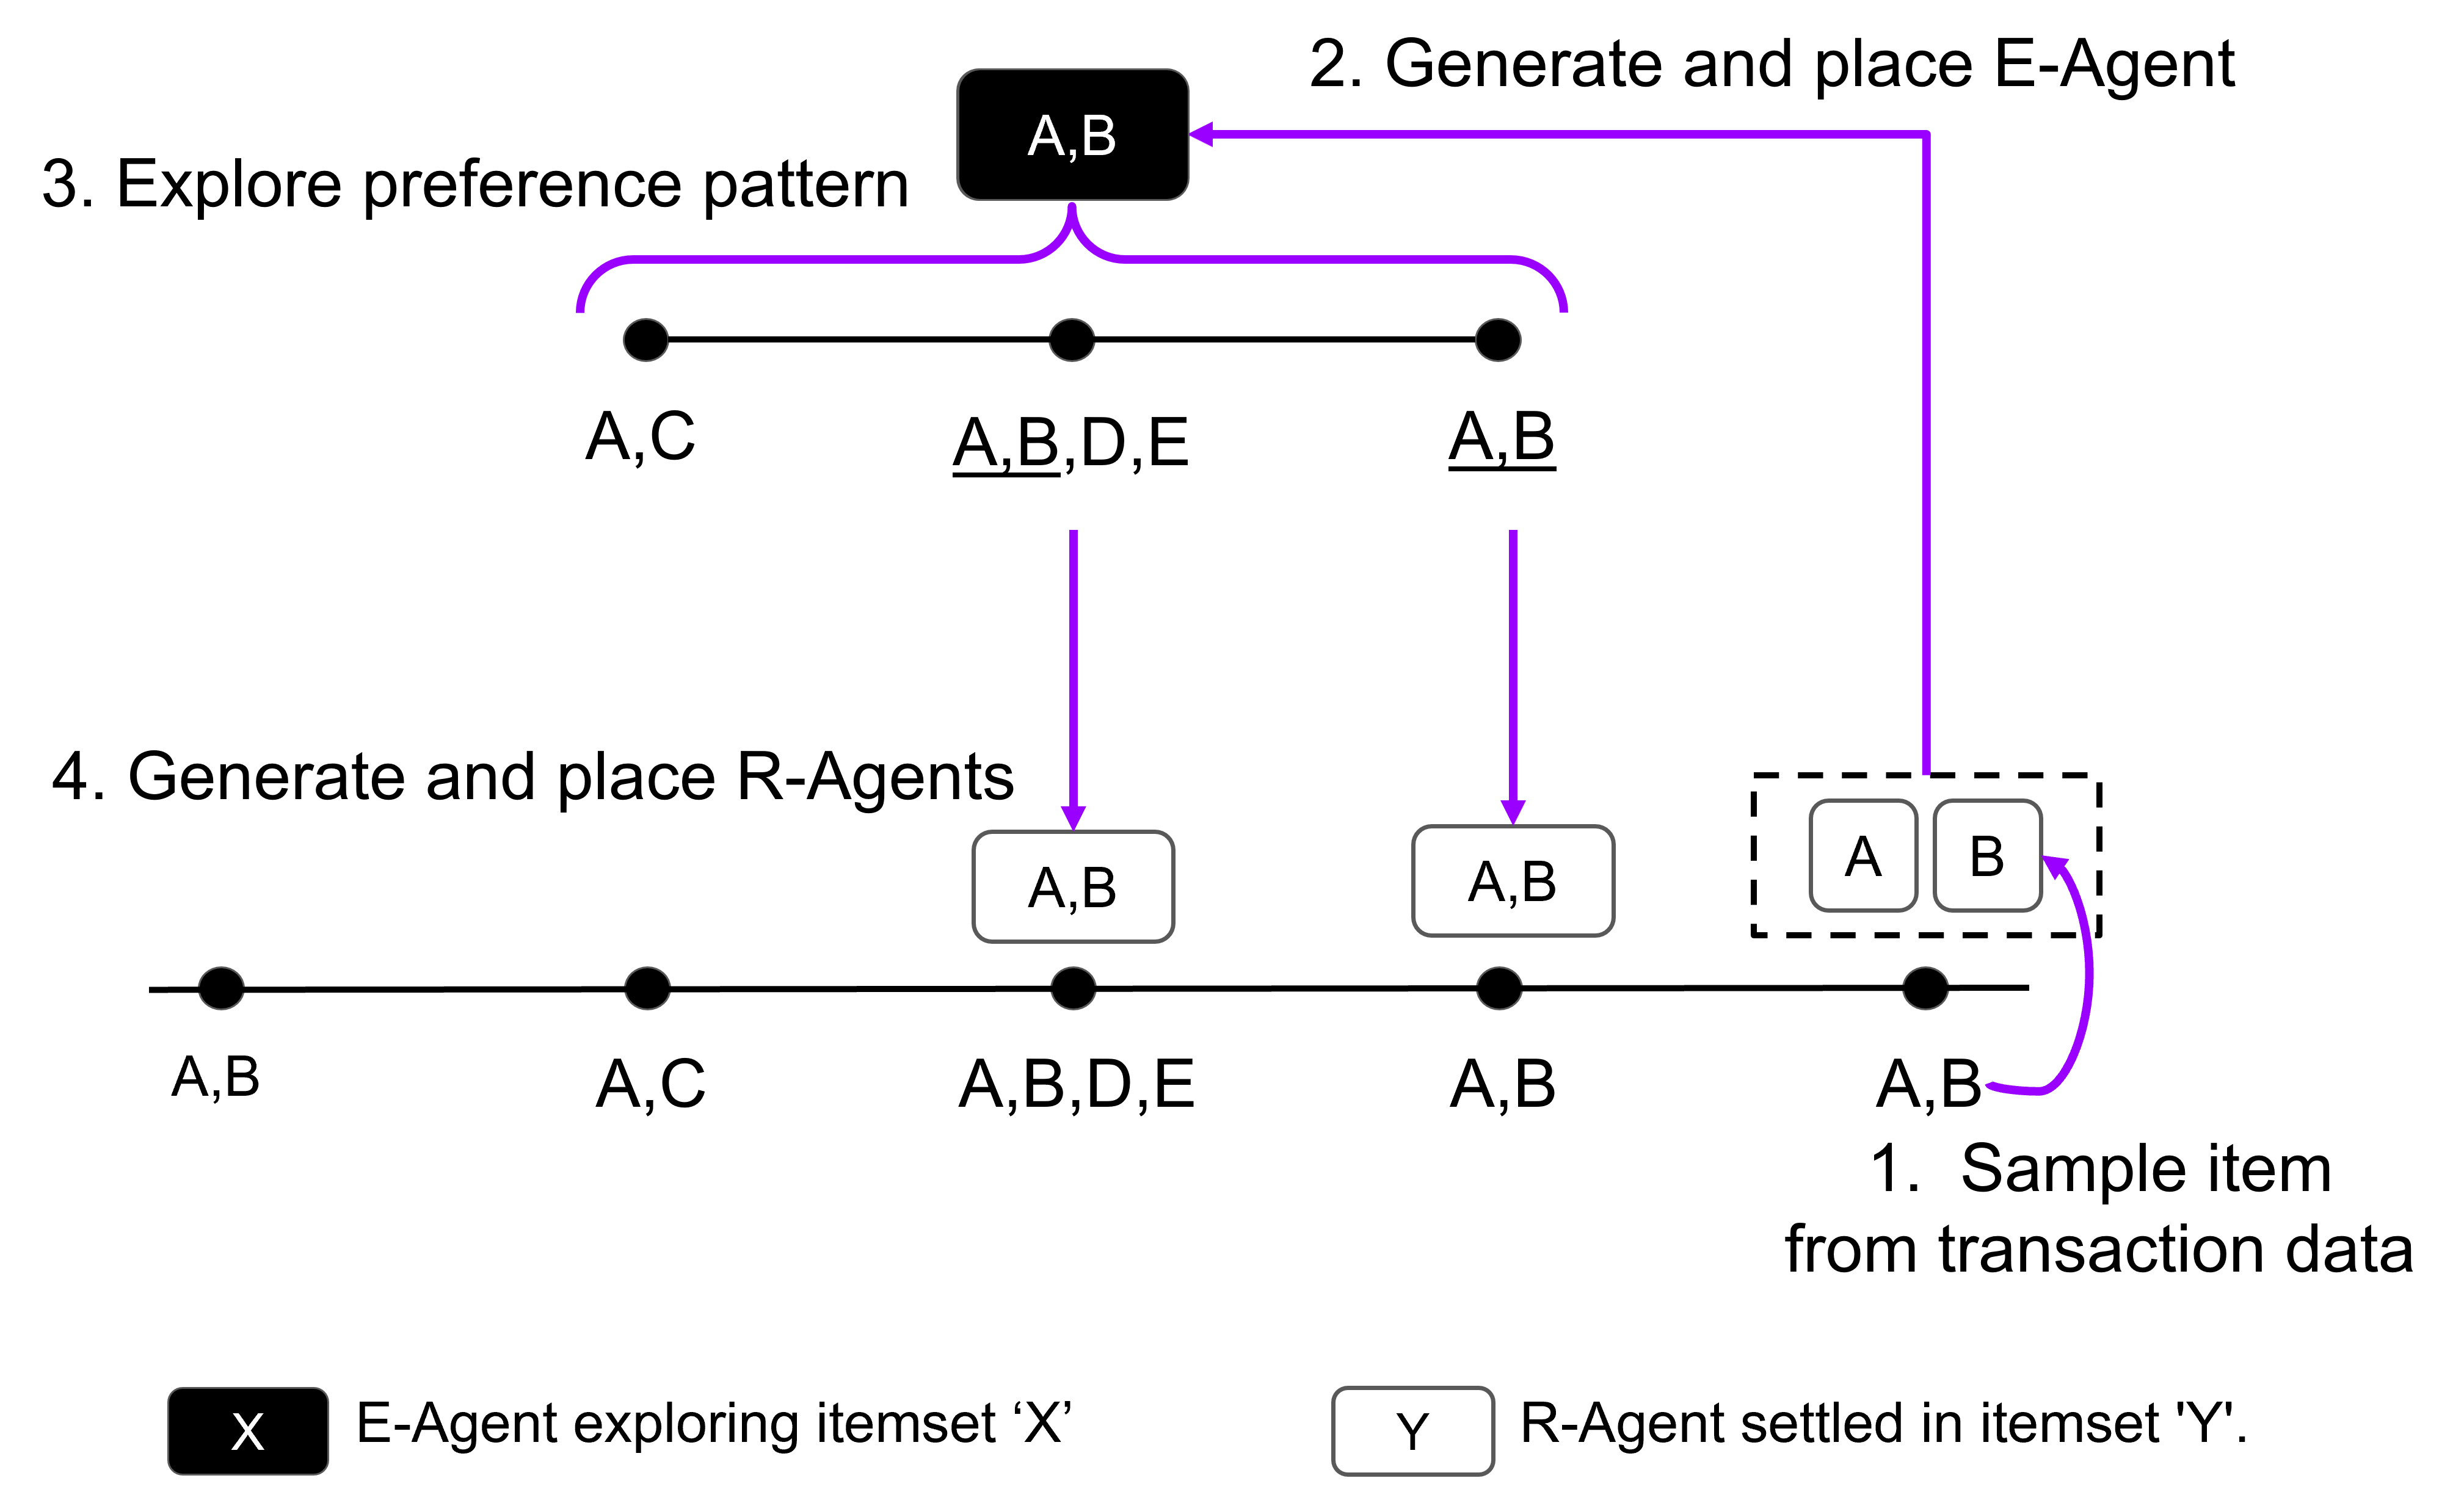
\includegraphics[width=1\linewidth]{fig/candidate-extraction-module.png}
    \caption{Behavior of the two types agent in the candidate extraction module. The strings written within each agent represent preference patterns.  After executing the steps 1 through 4, the distribution of R-Agents is aggregated and candidate patterns and their dense intervals are selected. This cycle is resumed after pattern identification in the pattern evaluation module.}
    \label{fig:candidate-extract}
\end{figure}

The objective of the candidate extraction module is to identify itemsets and corresponding concentrated intervals that are likely to be judged as dense patterns. To find these candidate patterns, the module takes a swarm intelligence-based bottom-up search approach. This approach is inspired by the behavior of plants that expand their habitat through hybridization. Specifically, the module finds itemsets that appear at dense intervals from other itemsets within the transaction to which the items sampled from transaction data belongs or nearby.

The candidate extraction module consists of two types of agents: \emph{R-Agents} (resident-agent) and \emph{E-Agents} (explore-agent). The R-Agent functions as a marker by indicating the transaction in which each item appears. The E-Agent, on the other hand, is responsible for searching for occurrences of the target item set within the transactions adjacent to the assigned timestamp.


In order to search for candidate patterns, the process is decomposed into several sequential steps, as shown in Fig.~\ref{fig:candidate-extract}. Initially, unit R-Agents are deployed using items randomly extracted from the dataset(step 1 in Fig.~\ref{fig:candidate-extract}). Each of these agents retains its respective item as a preference pattern, thereby serving as the starting point for subsequent exploration. 
Next, each R-Agent consults its own preference pattern along with that of neighboring R-Agents to determine the itemset to be explored in the next time step. The determined itemset is then set as the preference pattern for the E-Agents in the subsequent phase. This determination process adopts one of two modes: a replication mode, which preserves the current preference pattern unchanged, or a synthesis mode, which outputs the union of the preference patterns.E-Agents generated by the above process are probabilistically placed near the position of the parent R-Agent (step 2 in Fig.~\ref{fig:candidate-extract}).
Once deployed, these E-Agents actively search within a predetermined region for the occurrence of itemsets that match their preference patterns(step 3 in Fig.~\ref{fig:candidate-extract}). When an E-Agent detects a transaction containing the target itemset, it places a new R-Agent at that transaction(step 4 in Fig.~\ref{fig:candidate-extract}).

Finally, the number of R-Agents associated with each itemset is aggregated, and if this count exceeds a  minimum occurrence threshold($= minSup \times minL$), the corresponding itemset is selected as a candidate pattern. The spatial distribution of all R-Agents associated with the selected itemset is then defined as the candidate dense interval for that pattern.

After the pattern evaluation phase, the candidate extraction process is iteratively repeated. This cyclical generation ultimately results in the extraction of densely occurring patterns with localized concentrations, along with their corresponding dense intervals.
Itemsets that are determined to be dense patterns are suppressed from being selected as preferred patterns in the candidate extraction module. In this paper, we distinguish two variants of the Plant Model by their suppression strategy:
\begin{itemize}
  \item \emph{Plant Model (Global Suppression)}: Once an itemset is judged to be dense, its occurrences are suppressed across the entire transaction dataset.
  \item \emph{Plant Model (Interval‑Restricted Suppression)}: Suppression is applied only within the detected dense interval of the pattern.
\end{itemize}


\begin{algorithm}[t] 

    \makeatletter 
    \renewcommand{\algorithmicrequire}{\textbf{Input:}} 
    \renewcommand{\algorithmicensure}{\textbf{Output:}} 
    \makeatother
    
    \begin{algorithmic}[1]
    \caption{Candidate Extraction Module} 
    \label{alg:candidate-extraction-module}
        \Require Transaction data $D$, maximum pattern length $plength_{max}$, unit R-Agent number $pop_{btm}$, R-Agent sampling number $N_{sampling}$, exploration range radius $r$, scan waiting cycle count $w_{scan}$, replication probability $prob_{copy}$, tentative pattern candidate set $C_{tentative}$, E-Agents list $Agents_{explore}$, dense pattern set $L$, minimum occurrence threshold $minfreq$
        \Ensure List of pairs (pattern candidate, candidate region) $P$, tentative pattern candidate set $C_{tentative}$, E-Agents list $Agents_{explore}$
        
        \State $P \gets \{\}$ 
        % \Comment{Initialize the set of pattern candidates and their regions}

        \State $Agents_{resident} \gets \{\}$
        \State Generate and deploy unit R-Agents.
        \State Add the generated unit R-Agents to $Agents_{resident}$.
        
        \For{$Agent_{explore}$ \textbf{in} $Agents_{explore}$}
            \State Generate and deploy R-Agents.
            \State Add the generated R-Agents to $Agents_{resident}$.
        \EndFor
        
        \State Delete all E-Agents.
        \State Delete all R-Agents that have attempted the discovered dense patterns.
        \State Add itemsets with R-Agent count $\geq minfreq$ to $C_{tentative}$ 
        % \Comment{Record tentative pattern candidates}
        
        \For{$candidate$ \textbf{in} $C_{tentative}$}
            \If{the waiting cycle count of $candidate$ $\geq w_{scan}$}
                \State Add ($candidate$, list of occurrence positions) to $P$ 
                % \Comment{Record the pair of pattern candidate and candidate region}
            \Else
                \State the waiting cycle count of $candidate$ ++.
            \EndIf
        \EndFor
        
        \State Sample R-Agents.
        \For{$Agent_{resident}$ \textbf{in} $Agents_{resident(sampled)}$}
            \State Generate a new pattern $F_{new}$.
            \State Generate and deploy E-Agents.
            \State Add the generated E-Agents to $Agents_{explore}$.
        \EndFor
        
        \State Delete all R-Agents.
        
        \State \Return $P$, $C_{tentative}$, $Agents_{explore}$
    \end{algorithmic}
\end{algorithm}


\subsubsection{Pattern Evaluation Module}
% \input{alg/pattern_evaluation_module}

The pattern evaluation module is introduced to accurately extract truly dense patterns from the R-Agent location data produced by the candidate extraction module.
The input to the pattern evaluation module, denoted as \(positions\), is a sorted list of the R-Agents’ fixed positions corresponding to the transactions in which each candidate pattern occurs. The module applies a sliding window mechanism as well as Apriori-window over \(positions\) to detect dense intervals. 



\subsubsection{Termination Conditions}
In addition to termination by the predefined maximum iterations, the Plant Model introduces early termination. If no new dense patterns are extracted after the start of the run or after the last dense pattern is extracted for one-fifth of the maximum number of cycles, the model terminates early without waiting for the maximum iterations to elapse.

\subsubsection{Hyperparameters}
The attributes of the two types of agents and the number of agents produced are based on the hyperparameters listed in Table \ref{tab:plant_params}. Maximum Iterations defines the maximum number of cycles to be completed. No. of Unit R-Agents specifies the number of unit R-Agents generated in each cycle. R-Agent Sampling Count specifies the number of R-Agents that generate E-Agents. Exploration Range Radius specifies the range to be searched by each E-Agent. Scan Wait Cycle Count specifies the number of waiting cycles from the time a candidate is registered as a pattern candidate to the time it is evaluated. Replication Probability specifies the probability that a R-Agent chooses the replication mode when generating preference patterns.

\begin{table}[t]
    \centering
    \caption{Hyperparameters of Plant Model}
    \begin{tabular}{|c|c|}
        \hline
        \textbf{Hyperparameter} & \textbf{Description} \\
        \hline
        Maximum Iterations & 
        \begin{tabular}{@{}l@{}}
            The maximum number of cycles \\
            until termination
        \end{tabular} \\\hline
        No. of Unit R-Agents & 
        \begin{tabular}{@{}l@{}}
            The number of unit R-Agents \\
            generated in each epoch
        \end{tabular} \\\hline
        R-Agent Sampling Count &
        \begin{tabular}{@{}l@{}}
            The number of R-Agents available \\
            for generating exploratory agents
        \end{tabular} \\\hline
        Exploration Range Radius & 
        \begin{tabular}{@{}l@{}}
            The range within which \\
            the E-Agents search
        \end{tabular} \\\hline
        Scan Wait Cycle Count & 
        \begin{tabular}{@{}l@{}}
        The number of cycles to wait \\for pattern candidate registration
        \end{tabular} \\\hline
        Replication Probability &
        \begin{tabular}{@{}l@{}}
            The probability of selecting\\ the replication mode\\
            during preference pattern generation
        \end{tabular} \\
        \hline
    \end{tabular}
    \label{tab:plant_params}
\end{table}

\section{Experiments}
\label{sec:experiments}
% 実験の目的
The experiments were designed to evaluate the performance of our proposed method on real-world datasets, focusing on two key aspects: (1) the accuracy of dense pattern identification and (2) the accuracy of dense interval detection. To achieve this, we compare our approach with existing methods by introducing two novel evaluation metrics.
% 共通して用いるデータセットの説明
The datasets used in the experiments are publicly available and are often utilized as benchmarks in pattern mining research\cite{fournier2016spmf}. 

\begin{table}[t]
    \centering
    \begin{threeparttable}
    \caption{Statistical information of real-world datasets}
    \label{tab:dataset_stats}
    \begin{tabular}{|c|c|c|}
    \hline
    Dataset       & No. of transactions & No. of unique items \\
    \hline
    Retail        & 88,162              & 16,470               \\
    OnlineRetail  & 541,909*            & 4,070                \\
    Kosarak       & 990,002             & 41,270               \\
    ChicagoCrime  & 1,000,000           & 42,655               \\
    \hline
    \end{tabular}
    \begin{tablenotes}
        \small{\item *Deleted blank transactions in preprocessing}
    \end{tablenotes}
    \end{threeparttable}
\end{table}


\subsection{Experiment 1: Dense Pattern Identification}
% 尺度の導入
\subsubsection{Metrics}
To assess the accuracy of pattern identification, we use F1-score metrics the same as in the preliminary experiments.

% 正解データの用意
To compute the above metrics, we generate ground truth patterns for each dataset. For the Retail dataset, the ground truth is defined as the dense patterns that satisfy a $minL$ of 500 and a $minsup$ of 10\%. For the remaining datasets, the ground truth patterns are those meeting a $minL$ of 250 and a $minsup$ of 10\%. This ground truth is obtained using an extended version of the Apriori algorithm, an exact solution method that precisely extracts the patterns satisfying these conditions.

\subsubsection{Methods}
% 比較手法の紹介
We compare Plant Model (Global Suppression) to five baseline methods: Apriori\cite{agrawal1994fast}, PFPM\cite{tanbeer2009discovering}, PPFPM\cite{kiran2017discovering}, LPFIM\cite{mahanta2005finding}, and LPPM\cite{fournier2021mining}.
Apriori extracts itemsets that appear frequently in the entire data set. PFPM and PPFPM extract itemsets that appear periodically. Specifically, the former method extracts itemsets that are periodic across the entire data set, while the latter method relaxes the conditions to extract patterns that show periodicity in some parts of the data.
LPFIM and LPPM are methods for extracting both periodic itemsets and intervals that exhibit periodicity.


% パラメータの探索
\subsubsection{Parameters}
We perform a grid search per dataset to select both the baseline methods’ parameters and the Plant Model’s hyperparameters. For the baselines, we simply take the configuration that achieves the highest score within the search space. In principle, if the Plant Model is allowed unlimited computational cost, it will almost certainly generate agents matching every dense pattern—driving its F1‐score to 1. Therefore, in this experiment we choose hyperparameters that balance extraction accuracy against execution time. The search spaces and the specific parameter values used in the experiments for all methods are detailed in Appendix \ref{sec:params_space} and \ref{sec:params}.

% The same grid‐search procedure used in Experiment 1 for Plant Model (Global Suppression) was also applied to Plant Model (Interval‐Restricted Suppression), tuning its settings to balance the Jaccard score and runtime.

\subsubsection{Experimental Conditions}
All baseline methods are deterministic algorithms and thus each was run only once. Because Plant Model (Global Suppression) is stochastic, we performed 20 independent trials and report the mean F1‐score. 

\subsubsection{Results of Experiment 1}
\begin{table*}[t]
  \centering
  \begin{threeparttable}
    \caption{Pattern identification F1‐scores for each method and dataset}
    \label{tab:f1_scores}
    \begin{tabular}{|c|cccc|}
      \hline
      Method & Retail & OnlineRetail & Kosarak & ChicagoCrime \\
      \hline
      Apriori                   & 0.017 & 0.003 & * & 0.006 \\
      PFPM                      & 0.529 & 0.220 & 0.933      & 0.614 \\
      PPFPM                     & 0.863 & 0.573 & 0.933      & 0.740 \\
      LPFIM                     & 0.964 & 0.872 & 0.966      & 0.952 \\
      LPPM                      & 0.967 & 0.832 & \textbf{0.983} & \textbf{0.976} \\
      Plant Model (Global Suppression)          & \textbf{0.990} $\pm$ 0.008 & \textbf{0.980} $\pm$ 0.012& 0.955 $\pm$ 0.030 & 0.974 $\pm$ 0.013\\
      \hline
    \end{tabular}
    \begin{tablenotes}
      \footnotesize
      \item[*] Apriori was terminated after running for approximately one week on the Kosarak dataset without producing any results, so no score was recorded.
    \end{tablenotes}
  \end{threeparttable}
\end{table*}

Table \ref{tab:f1_scores} shows that among the deterministic baselines, LPPM achieves the highest F1-score on Kosarak (0.983) and ChicagoCrime (0.976), with LPFIM slightly behind. PFPM and PPFPM deliver moderate performance, while Apriori fails to complete on Kosarak. Plant Model (Global Suppression) surpasses all baselines on Retail and OnlineRetail—reaching 0.990 $\pm$ 0.008 and 0.980 $\pm$ 0.012, respectively—and remains highly competitive on ChicagoCrime (0.974 $\pm$ 0.013). Although its score on Kosarak (0.955 $\pm$ 0.030) falls short of LPPM’s, Plant Model exhibits overall consistency across datasets and its ability to maintain top‑tier accuracy.
In particular, Plant Model (Global Suppression) was significantly more accurate for Retail and OnlineRetail ($p<0.01$).
This accuracy gain stems from its robustness to variable occurrence intervals. Table \ref{tab:dataset_std} quantifies this variability per dataset by averaging the standard deviation of each item set’s densest (least variable) interval—since those intervals drive dense‑pattern extraction—and shows that OnlineRetail’s variability is roughly three times higher than the others.
Conventional methods must raise the maximum‑interval threshold to cover diverse gaps, which lowers detected‑interval density and causes false positives and misses (as our preliminary experiments confirm). In contrast, the Plant Model’s sliding‑window evaluation needs no such threshold, so density remains constant despite interval variability, yielding stable, high‑precision extraction.



\begin{table}[t]
    \centering
    \caption{Variation in occurrence intervals for each dataset}
    \begin{tabular}{|c|c|}
        \hline
        Dataset & 
        \begin{tabular}{c}
            \scriptsize{Mean of minimum standard deviations} \\ 
            \scriptsize{of occurrence intervals}
        \end{tabular} \\\hline
        Retail & 7.31 \\
        OnlineRetail & 20.51 \\
        Kosarak & 6.12 \\
        ChicagoCrime & 6.95 \\
        \hline
    \end{tabular}
    \label{tab:dataset_std}
\end{table}

\begin{table}[t]
    \centering
    \caption{Average number of occurrences of top 20 items in each dataset}
    \begin{tabular}{|c|c|}
        \hline
        Dataset & Average occurrences of top 20 items \\ \hline
        Retail         & 8,917.25   \\
        OnlineRetail   & 29,706.70  \\
        Kosarak        & 120,358.25 \\
        ChicagoCrime  & 237,506.85 \\ \hline
    \end{tabular}
    \label{tab:itemcount}
\end{table}


% \subsubsection{Discussion.}

\subsection{Experiment 2: Dense Interval Detection}
\subsubsection{Metrics}
For dense interval detection accuracy, the similarity between the ideal dense intervals and those detected by the method is evaluated using the Jaccard coefficient defined in Equation (\ref{eq:Jaccard}). For a given itemset \(X\), let \(A\) denote the set of all timestamps within the ideal dense intervals and \(B\) denote the set of all timestamps within the dense intervals detected by the method.

\begin{IEEEeqnarray}{rCl}
J_X(A,B) & = & \frac{\lvert A\cap B\rvert}{\lvert A\cup B\rvert}\,. 
\label{eq:Jaccard}
\end{IEEEeqnarray}

The overall dense interval detection performance is then assessed by computing the mean Jaccard coefficient over all true dense patterns, where a value closer to 1 indicates higher accuracy. Ground‑truth dense sections are detected using the same method as in Experiment 1. Erroneous inclusion of non‑dense timestamps increases $\lvert A\cup B\rvert$. Omission of true dense timestamps decreases $\lvert A\cap B\rvert$. Both types of error lead to a reduced Jaccard coefficient. This clarifies how over‑ and under‑detection affect detection accuracy.


\subsubsection{Methods}
We compare the interval‑detection accuracy of two Plant Model variants—Plant Model (Global Suppression) and Plant Model (Interval‑Restricted Suppression)—against two baseline interval‑extraction methods, LPFIM and LPPM. LPFIM and LPPM serve as representative approaches for periodic interval detection. All methods use the same parameter settings as in Experiment 1.

\subsubsection{Parameters}
LPFIM, LPPM, and Plant Model (Global Suppression) use the same parameters as in Experiment 1.  
We applied the Experiment 1 grid search to Plant Model (Interval‑Restricted Suppression), selecting hyperparameters that balance F1-score and runtime.

\subsubsection{Experimental conditions}
As in Experiment 1, each baseline method was run once. Both Plant Model variants were run ten times, and the mean Jaccard coefficient across runs was used for comparison. 


\subsubsection{Results of Experiment 2}

\begin{table*}[t]
  \centering
  \caption{Jaccard coefficients for dense interval detection. }
  \label{tab:jaccard_scores}
  \begin{tabular}{|c|cccc|}
    \hline
    Method & Retail & OnlineRetail & Kosarak & ChicagoCrime \\
    \hline
    LPFIM                                    & 0.674 & 0.072 & 0.104 & 0.501 \\
    LPPM                                     & 0.811 & 0.213 & 0.324 & 0.545 \\
    Plant Model (Global Suppression)                        &  0.590 $\pm$ 0.032 & 0.738 $\pm$ 0.032& 0.090 $\pm$0.036 & 0.268 $\pm$ 0.026 \\
    Plant Model (Interval‑Restricted Suppression)                       & \textbf{0.984} $\pm$ 0.005& \textbf{0.987} $\pm$0.008& \textbf{0.621}$\pm$ 0.027& \textbf{0.867}$\pm$ 0.019\\
    \hline
  \end{tabular}
\end{table*}


\begin{figure*}[t]
  \centering
  %============ Retail ============%
  \begin{subfigure}[t]{\textwidth}
    \centering
    \begin{subfigure}[b]{0.48\textwidth}
      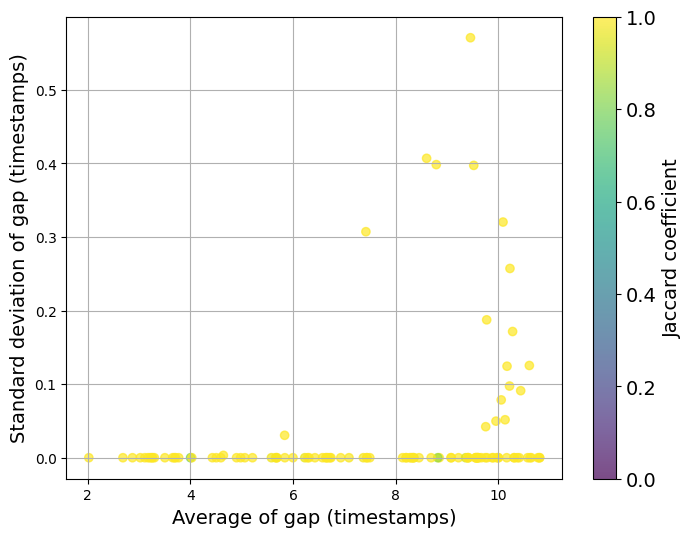
\includegraphics[width=\linewidth]{fig/retail_plant_plus_best_params.png}
      \caption{Plant Model (Interval‑Restricted Suppression)}
      \label{fig:retail_interval_restricted}
    \end{subfigure}
    \hfill
    \begin{subfigure}[b]{0.48\textwidth}
      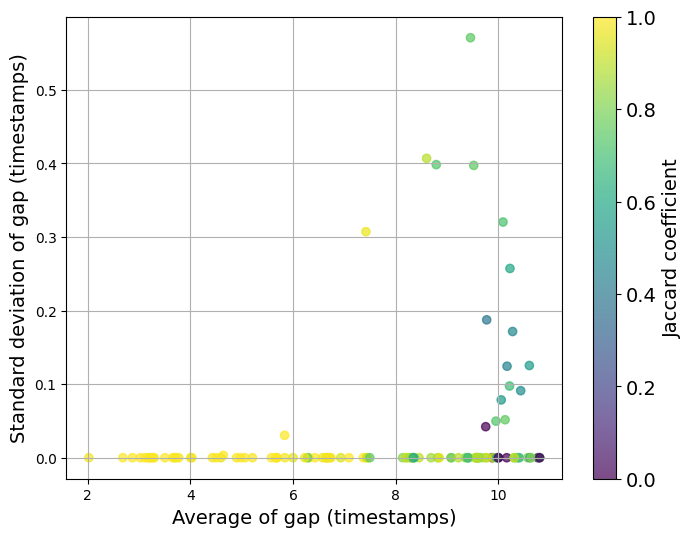
\includegraphics[width=\linewidth]{fig/retail_lppm_best_params.png}
      \caption{LPPM}
      \label{fig:retail_lppm}
    \end{subfigure}
    \label{fig:retail_jaccard}
  \end{subfigure}

  \caption{Jaccard coefficients for dense patterns in Retail. Each point represents an itemset: the x‑axis shows the mean occurrence gap, and the y‑axis shows the gap’s standard deviation. In this experiment, timestamps are recorded at fixed intervals. A coefficient closer to 1 denotes more accurate interval extraction.}
  \label{fig:jaccard_by_pattern}
\end{figure*}


Table~\ref{tab:jaccard_scores} highlights the limitations of periodic pattern mining methods: the Jaccard coefficients of LPFIM range from only 0.072 (OnlineRetail) to 0.674 (Retail), and although LPPM improves on these (0.213–0.811), it still misses or misdetects many of the true dense intervals. Plant Model (Global Suppression) falls even below these baselines because suppressing agent generation across all intervals prevents sufficient coverage. In contrast, the Plant Model (Interval-Restricted Suppression) shows better Jaccard coefficients than any other method because it keeps 
agents extracting candidates until nearly all dense intervals have been detected.

Fig. \ref{fig:jaccard_by_pattern} shows the Jaccard coefficient for each dense itemset in Retail dataset. LPPM achieves low interval detection accuracy for patterns with large average gaps and large gap variation, while the Plant Model (Interval-Restricted Suppression) maintains high Jaccard coefficients in exactly such difficult cases The results demonstrate that the Jaccard coefficient remains high even in such difficult cases. 


\subsection{Discussion}
% \begin{figure}[t]
%     \centering
%     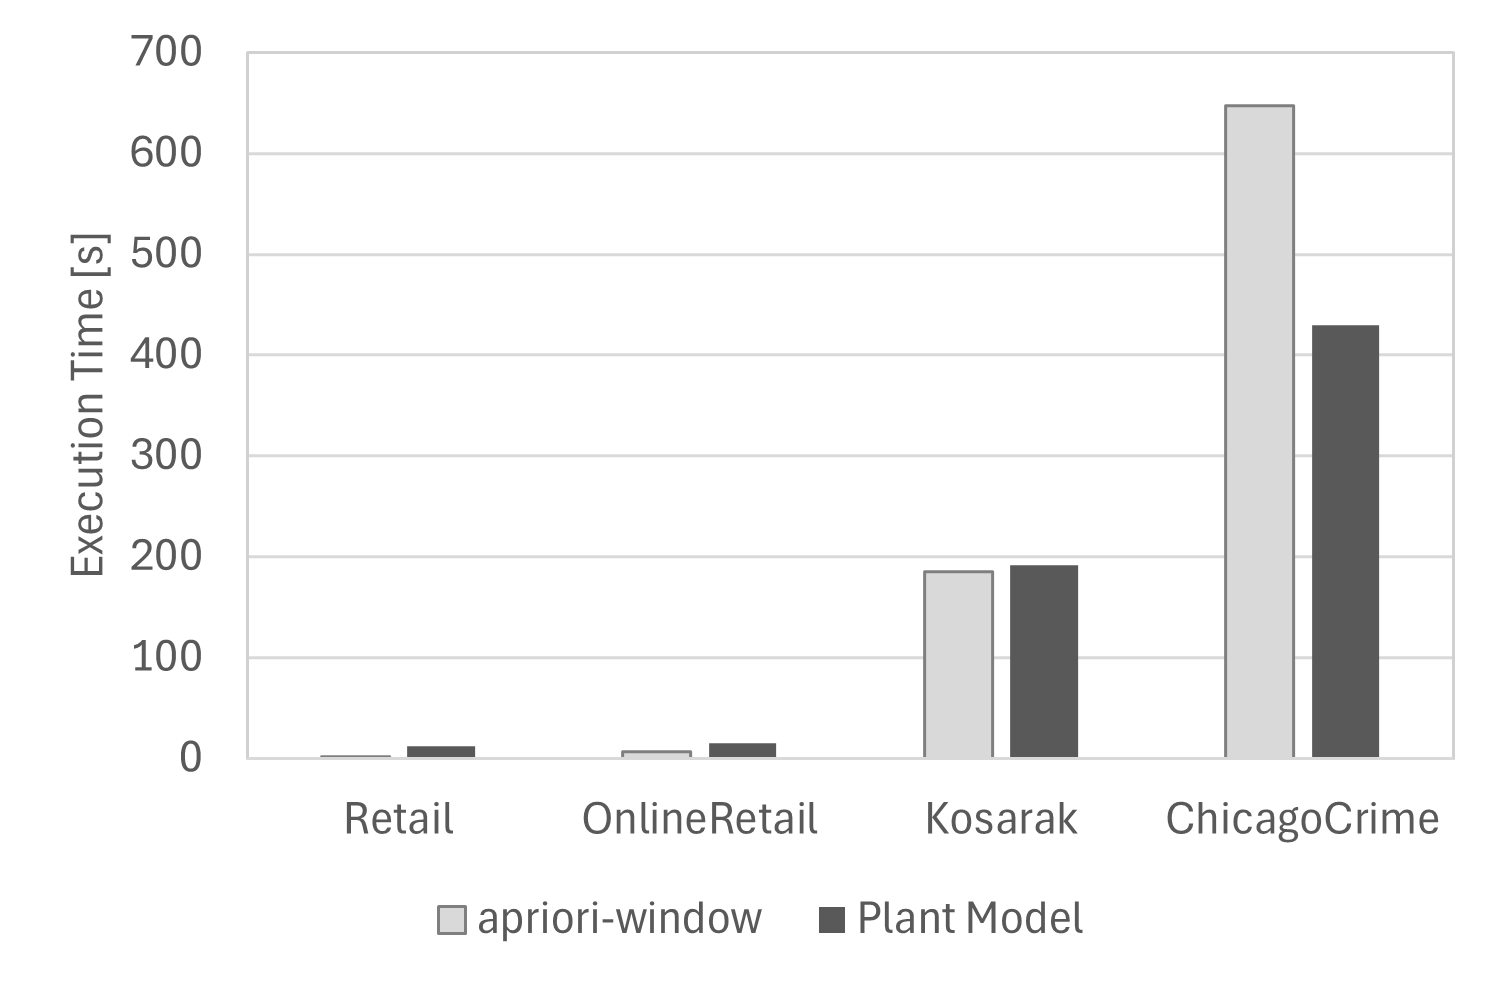
\includegraphics[width=1\linewidth]{fig/execution_time.png}
%     \caption{Execution time for Apriori‑window and both Plant Model variants.}
%     \label{fig:execution_time}
% \end{figure}

\begin{table*}[t]
\centering
\caption{Execution times (seconds) on various datasets}
\label{tab:exec-times}
\begin{tabular}{|c|cccc|}
\hline
\textbf{Method} & \textbf{Retail} & \textbf{OnlineRetail} & \textbf{Kosarak} & \textbf{ChicagoCrime} \\
\hline
Apriori-window & 1.62 & 6.63   & 185.73  & 647.53  \\
Plant Model (Global Suppression)           & 12.45  & 14.70  & 191.61  & 429.71  \\
Plant Model (Interval Restricted Suppression) & 138.68 & 114.22 & 3108.73 & 1433.24 \\
\hline
\end{tabular}
\end{table*}



We discuss the trade-off between accuracy and execution time for the proposed set of methods.
Table~\ref{tab:exec-times} compares execution times for Apriori‑window, Plant Model (Global Suppression), and Plant Model (Interval‑Restricted Suppression). 
All methods were implemented in Rust and executed on a Windows 11 Home 64‑bit PC with 32GB RAM and an AMD Ryzen 7 5700X (3.4GHz, 8cores/16threads).
For Retail and OnlineRetail, Apriori‑window remains fastest. On the larger Kosarak and ChicagoCrime datasets, Plant Model (Global Suppression) runs as fast as—or faster than—Apriori‑window.

As indicated by the execution time results in Experiment 1, Plant Model (Global Suppression) achieves a higher F1-score on ChicagoCrime with a shorter execution time than Apriori‑window, suggesting that its sampling strategy locates dense patterns very quickly. However, Experiment 2 shows that this variant attains lower interval‑detection accuracy than the baselines.

In contrast, Plant Model (Interval‑Restricted Suppression) delivers high Jaccard coefficients in Experiment 2, confirming precise extraction of dense intervals. Its execution times on the Retail, OnlineRetail, Kosarak, and ChicagoCrime datasets were 138.68s, 114.22s, 3108.73s, and 1433.24s, respectively, all exceeding those of both Apriori‑window and Plant Model (Global Suppression). Therefore, improving the time efficiency of this variant remains an important challenge.


\section{Conclusion}
\label{conclusion}
This study addressed the task of extracting dense patterns by introducing two complementary approaches: Apriori‑window, an exact algorithm that exhaustively identifies all dense patterns, and Plant Model, a heuristic method with two suppression strategies. The Global Suppression variant of Plant Model demonstrated superior pattern‑identification accuracy and runtime efficiency but showed reduced precision in detecting the exact intervals. In contrast, the Interval‑Restricted Suppression variant enhanced the interval‑detection accuracy, albeit with a decrease in computational efficiency. 

Future research should include hyperparameter tuning that adapts to the characteristics of each dataset and improves the accuracy of the interval extraction. The process of tuning hyperparameters currently requires iterative application, placing a heavy burden on the user. Hence, an automatic parameter adjustment strategy would be highly beneficial, minimizing user intervention and improving the algorithm’s practical utility. Additionally, since the Plant Model improves the accuracy of dense interval extraction by relaxing agent suppression conditions but also increases execution time, we aim to spread agents efficiently within dense intervals by modifying the algorithm.

Another promising extension lies in extracting patterns at various temporal scales (e.g., hour, day, week) from large transaction datasets. The proposed methods can handle diverse interval lengths by adjusting the width of the sliding window. Implementing multiple sliding windows would make it possible to capture patterns across different time scales within large datasets, which could further advance knowledge discovery. 

\section*{Acknowledgment}
The authors acknowledge that portions of the text in this paper were generated with OpenAI’s large language model ChatGPT.




\bibliographystyle{IEEEtran.bst}
\bibliography{refs}

\newpage
\appendices
\section{Parameter Search Procedures}
\label{sec:params_space}
For each method and dataset, a grid search was performed over the specified parameter ranges. Deterministic methods (PFPM, PPFPM, LPFIM, LPPM) use single‐run F1-scores; stochastic methods (both Plant Model variants) use the mean F1-score over five independent runs. Any configuration whose runtime exceeded one hour was excluded.

\subsection{PFPM}
A progressively narrowing search strategy was applied to the maximum allowable gap (gap) parameter.The overall search space was defined as follows.

\begin{itemize}
  \item Retail: gap\(\in[50,900]\)
  \item OnlineRetail: gap\(\in[100,3500]\)
  \item Kosarak: gap\(\in[50,450]\)
  \item ChicagoCrime: gap\(\in[1000,10000]\)
\end{itemize}

First, a coarse search was conducted over all datasets, evaluating at increments of 50 for Retail, 100 for OnlineRetail, 50 for Kosarak, and 1000 for ChicagoCrime. Next, for Retail and Kosarak, the provisional optimal gap from the coarse search was re-evaluated within a ±50 range at 10-unit increments, and for OnlineRetail, within a ±100 range at 10-unit increments. For ChicagoCrime, a finer-grained search was performed: an intermediate search around the coarse optimal gap within a ±1000 range at 100-unit increments was followed by a fine-tuning search around the intermediate optimal gap within a ±100 range at 10-unit increments.


\subsection{PPFPM}
A simultaneous grid search was conducted over the maximum allowable gap and the periodic ratio parameters. The overall search space was defined as follows.
Both parameters were varied at 10‑unit increments across their respective ranges for each dataset.

\begin{itemize}
  \item Retail: gap\(\in[10,200]\), ratio\(\in[10,100]\)
  \item OnlineRetail: gap\(\in[10, 500]\), ratio\(\in[10,100]\)
  \item Kosarak: gap\(\in[10,500]\), ratio\(\in[10,100]\)
  \item ChicagoCrime: gap\(\in[10,900]\), ratio\(\in[10,100]\)
\end{itemize}


\subsection{LPFIM}
A grid search over all hyperparameter combinations was performed in 5‐unit increments. The evaluated ranges for each dataset were as follows:
\begin{itemize}
  \item Retail: minsup $\in[10,50]$, max gap $\in[10,120]$, min\_interval\_size $\in[100,700]$.
  \item OnlineRetail: minsup $\in[10,50]$, max gap $\in[5,1000]$, min\_interval\_size $\in[10,500]$.
  \item Kosarak: minsup $\in[10,50]$, max gap $\in[5,500]$, min\_interval\_size $\in[50,500]$.
  \item ChicagoCrime: minsup $\in[10,50]$, max gap $\in[5,750]$, min\_interval\_size $\in[50,500]$.
\end{itemize}

\subsection{LPPM}
A full grid search in 5‐unit increments was carried out over all three LPPM parameters for each dataset. The evaluated ranges for each dataset were as follows.  :
\begin{itemize}
  \item Retail: maxPer $\in[5,50]$, minDur $\in[5,1000]$, maxSoPer $\in[5,500]$.
  \item OnlineRetail: maxPer $\in[5,50]$, minDur $\in[5,500]$, maxSoPer $\in[5,500]$.
  \item Kosarak: maxPer $\in[5,50]$, minDur $\in[5,1600]$, maxSoPer $\in[5,500]$.
  \item ChicagoCrime: maxPer $\in[5,50]$, minDur $\in[5,500]$, maxSoPer $\in[5,500]$.
\end{itemize}

\subsection{Plant Model (Global Suppression)}
Parameters were searched over the combinations below. For each configuration, five independent runs were executed and the mean F1-score was recorded. Among those whose runtime approached that of Apriori‑window, the setting with the highest mean F1-score was selected.
\begin{itemize}
  \item Retail:
    \begin{itemize}
      \item Max Iterations: [25, 75, 150]
      \item No. of Unit R‑Agents: [2500, 7500, 15000]
      \item R‑Agent Sampling Count: [1500, 7500, 15000]
      \item Exploration Range Radius: [10, 50, 100]
      \item Scan Wait Cycle Count: [1, 2]
      \item Replication Probability: [0.1, 0.3]
    \end{itemize}
  \item OnlineRetail:
    \begin{itemize}
      \item Max Iterations: [25, 50, 75]
      \item No. of Unit R-Agents: [25000, 50000, 100000]
      \item R-Agent Sampling Count: [250000, 500000, 1000000]
      \item Exploration Range Radius: [10, 30, 50]
      \item Scan Wait Cycle Count: [1, 2]
      \item Replication Probability: [0.1, 0.3]
    \end{itemize}
  \item Kosarak:
    \begin{itemize}
      \item Max Iterations: [25, 50, 75]
      \item No. of Unit R-Agents: [15000, 30000, 50000]
      \item R-Agent Sampling Count: [100000, 250000, 500000]
      \item Exploration Range Radius: [50, 125, 250]
      \item Scan Wait Cycle Count: [1, 2]
      \item Replication Probability: [0.1, 0.3]
    \end{itemize}
  \item ChicagoCrime:
    \begin{itemize}
      \item Max Iterations: [100, 150, 175]
      \item No. of Unit R-Agents: [50000, 75000]
      \item R-Agent Sampling Count: [100000, 200000]
      \item Exploration Range Radius: [50, 75, 100]
      \item Scan Wait Cycle Count: [1]
      \item Replication Probability: [0.1, 0.3]
    \end{itemize}
\end{itemize}

\subsection{Plant Model (Interval-Restricted Suppression)}
A grid search was performed over the same ranges. Each configuration was run five times, and the mean F1-score was used for evaluation. 
\begin{itemize}
  \item Retail:
    \begin{itemize}
      \item Max Iterations: [25, 75, 150]
      \item No. of Unit R-Agents: [2500, 7500, 15000]
      \item R-Agent Sampling Count: [1500, 7500, 15000]
      \item Exploration Range Radius: [10, 50, 100]
      \item Scan Wait Cycle Count: [1, 2]
      \item Replication Probability: [0.1, 0.3]
    \end{itemize}
  \item OnlineRetail:
    \begin{itemize}
      \item Max Iterations: [25, 50, 75]
      \item No. of Unit R-Agents: [25000, 50000, 100000]
      \item R-Agent Sampling Count: [250000, 500000, 1000000]
      \item Exploration Range Radius: [10, 30, 50]
      \item Scan Wait Cycle Count: [1, 2]
      \item Replication Probability: [0.1, 0.3]
    \end{itemize}
  \item Kosarak:
    \begin{itemize}
      \item Max Iterations: [25, 50, 75]
      \item No. of Unit R-Agents: [10000, 30000]
      \item R-Agent Sampling Count: [100000, 250000]
      \item Exploration Range Radius: [50, 125, 250]
      \item Scan Wait Cycle Count: [1]
      \item Replication Probability: [0.1]
    \end{itemize}
  \item ChicagoCrime:
    \begin{itemize}
      \item Max Iterations: [100, 150, 175]
      \item No. of Unit R-Agents: [50000, 75000]
      \item R-Agent Sampling Count: [100000, 200000]
      \item Exploration Range Radius: [10, 30, 50]
      \item Scan Wait Cycle Count: [1]
      \item Replication Probability: [0.1, 0.3]
    \end{itemize}
\end{itemize}

\section{Parameter in Experiments}
\label{sec:params}
\subsection{Apirori}
\begin{itemize}
    \item minsup = 10 for all datasets.
\end{itemize}

\subsection{PF}
\begin{itemize}
  \item Retail: minsup = 50, max gap = 170
  \item OnlineRetail: minsup = 25, max gap = 1170
  \item Kosarak: minsup = 25, max gap = 280
  \item ChicagoCrime: minsup = 25, max gap = 5450
\end{itemize}

\subsection{PPF}
\begin{itemize}
  \item Retail: minsup = 50, max gap = 20, ratio = 70
  \item OnlineRetail: minsup = 25, max gap = 35, ratio = 50
  \item Kosarak: minsup = 25, max gap = 280, ratio = 100
  \item ChicagoCrime: minsup = 25, max gap = 10, ratio = 20
\end{itemize}

\subsection{LPFIM}
These parameters were set in Experiments 1 and 2, but the max gap was changed in the preliminary experiments.
\begin{itemize}
  \item Retail: minsup = 10, max gap = 30, min interval size = 275
  \item OnlineRetail: minsup = 50, max gap = 5,  min interval size = 20
  \item Kosarak: minsup = 10, max gap = 15, min interval size = 110
  \item ChicagoCrime: minsup = 10, max gap = 30, min interval size = 170
\end{itemize}

\subsection{LPPM}
\begin{itemize}
  \item Retail: maxPer = 10, minDur = 425, maxSoPer = 105
  \item OnlineRetail: maxPer = 5,  minDur = 50,  maxSoPer = 55
  \item Kosarak: maxPer = 15, minDur = 305, maxSoPer = 20
  \item ChicagoCrime: maxPer = 10, minDur = 145, maxSoPer = 50
\end{itemize}

\subsection{Plant Model (Global Suppression)}
\begin{itemize}
  \item Retail: Max Iterations = 25, unit R‑Agents = 15000, sampling count = 15000, exploration range radius = 100, scan wait cycle count = 1, replication probability = 0.3
  \item OnlineRetail: Max Iterations = 50, unit R‑Agents = 50000, sampling count = 1000000, exploration range radius = 30, scan wait cycle count = 2, replication probability = 0.1
  \item Kosarak: Max Iterations = 75, unit R‑Agents = 15000, sampling count = 250000, exploration range radius = 50, scan wait cycle count = 2, replication probability = 0.1
  \item ChicagoCrime: Max Iterations = 175, unit R‑Agents = 75000, sampling count = 200000, exploration range radius = 75, scan wait cycle count = 1, replication probability = 0.1
\end{itemize}

\subsection{Plant Model (Interval-Restricted Suppression)}
\begin{itemize}
  \item Retail: Max Iterations = 150, unit R‑Agents = 15000, sampling count = 15000, exploration range radius = 100, scan wait cycle count = 2, replication probability = 0.3
  \item OnlineRetail: Max Iterations = 50, unit R‑Agents = 100000, sampling count = 250000, exploration range radius = 30, scan wait cycle count = 1, replication probability = 0.3
  \item Kosarak: Max Iterations = 75, unit R‑Agents = 30000, sampling count = 250000, exploration range radius = 125, scan wait cycle count = 1, replication probability = 0.1
  \item ChicagoCrime: Max Iterations = 175, unit R‑Agents = 50000, sampling count = 200000, exploration range radius = 50, scan wait cycle count = 1, replication probability = 0.3
\end{itemize}


\end{document}
